\documentclass[12pt,english,ignorenonframetext,]{beamer}

%%%%%%%%%%%%%%%
%% Beamer theme
% choose one from http://deic.uab.es/~iblanes/beamer_gallery/
% or http://www.hartwork.org/beamer-theme-matrix/
% \usetheme{Warsaw}
\usetheme{CambridgeUS}

%%%%%%%%%%%%%%%%%%%%%%
%% Beamer color theme
%% default albatross beaver beetle crane dolphin dove fly lily
%% orchid rose seagull seahorse whale wolverine

%\usecolortheme{seahorse}  %% very lighty
\usecolortheme{dolphin}    %% nice blue
\usecolortheme{orchid}     %% dark red ?
\usecolortheme{whale}      %% black and blue as Warsaw

%%%%%%%%%%%%%%%%%%%%%%%%%%%%%%%%%%%%%%%%%%%%%%%%%%%%%%%%%%%%%%%%%%%%%%%%%%%%%%%%
%% Define your own colors
\definecolor{blackblue}{rgb}{19,19,59}  % rgb(48,48,150)

%%%%%%%%%%%%%%%%%%%%%%%%%%%%%%%%%%%%%%%%%%%%%%%%%%%%%%%%%%%%%%%%%%%%%%%%%%%%%%%%
%% Change the theme
%\setbeamercolor{alerted text}{fg=orange}
%\setbeamercolor{background canvas}{bg=white}
%\setbeamercolor{block body alerted}{bg=normal text.bg!90!black}
%\setbeamercolor{block body}{bg=normal text.bg!90!black}
%\setbeamercolor{block body example}{bg=normal text.bg!90!black}
%\setbeamercolor{block title alerted}{use={normal text,alerted text},fg=alerted text.fg!75!normal text.fg,bg=normal text.bg!75!black}
%\setbeamercolor{block title}{bg=blue}
%\setbeamercolor{block title example}{use={normal text,example text},fg=example text.fg!75!normal text.fg,bg=normal text.bg!75!black}
%\setbeamercolor{fine separation line}{}
\setbeamercolor{frametitle}{fg=black}
%\setbeamercolor{item projected}{fg=black}
%\setbeamercolor{normal text}{bg=black,fg=yellow}
%\setbeamercolor{palette sidebar primary}{use=normal text,fg=normal text.fg}
%\setbeamercolor{palette sidebar quaternary}{use=structure,fg=structure.fg}
%\setbeamercolor{palette sidebar secondary}{use=structure,fg=structure.fg}
%\setbeamercolor{palette sidebar tertiary}{use=normal text,fg=normal text.fg}
%\setbeamercolor{section in sidebar}{fg=brown}
%\setbeamercolor{section in sidebar shaded}{fg= grey}
\setbeamercolor{separation line}{}
%\setbeamercolor{sidebar}{bg=red}
%\setbeamercolor{sidebar}{parent=palette primary}
%\setbeamercolor{structure}{bg=black, fg=green}
%\setbeamercolor{subsection in sidebar}{fg=brown}
%\setbeamercolor{subsection in sidebar shaded}{fg= grey}
%\setbeamercolor{title}{fg=blackblue}
%\setbeamercolor{titlelike}{fg=blackblue}


%%%%%%%%%%%%%%%%%%%%%%%
%% Other beamer options
%\setbeamercovered{transparent}
% Permet de laisser en gris le texte qui n'est pas encore apparu (lorsqu'on utilise les commandes avec des <1,2> ou <4-9>.

%\setbeamercolor{normal text}{fg=black,bg=white}

%%%%%%%%%%%%%%%%%%%%%%%
%% Change Beamer fonts
% \usefonttheme{default}
% \usefonttheme[onlymath]{serif}
\usefonttheme{serif}

\setbeamerfont{title}{family=\rm}
\setbeamerfont{titlelike}{family=\rm}
\setbeamerfont{frametitle}{family=\rm}

%%%%%%%%%%%%%%%%%%%%%%%%%%%%%%%%%%%%%%%%%%%%%%%%%%%%%%%%%%%%%%%%%%%%%%%%%%%%%%%%
%% innertheme
%% rectangles circles inmargin rounded
% \useinnertheme{rounded}  % XXX My preference
\useinnertheme{circles}    % XXX
\usepackage{amsmath}
\usepackage{setspace}

%%%%%%%%%%%%%%%%%%%%%%%%%%%%%%%%%%%%%%%%%%%%%%%%%%%%%%%%%%%%%%%%%%%%%%%%%%%%%%%%
%% outertheme
%% infolines miniframes shadow sidebar smoothbars smoothtree split tree
%\useoutertheme{infolines}

%% No navigation symbol.
\setbeamertemplate{navigation symbols}{}
\beamertemplatenavigationsymbolsempty

% XXX Add a background image to the slides
% \usepackage{tikz}
% \setbeamertemplate{background}{\includegraphics[width=\paperwidth,height=\paperheight,keepaspectratio]{IETR.jpg}}
% \setbeamertemplate{background}{{\centering\begin{tikzpicture}\node[opacity=0.15]{\includegraphics[width=0.98\paperwidth]{IETR_et_partenaires_IETR.png}};\end{tikzpicture}}}

% Other options
%\setbeamertemplate{footline}[page number]

\beamertemplateballitem
\setbeamertemplate{itemize item}[square]


\setbeamertemplate{caption}[numbered]
\setbeamertemplate{caption label separator}{: }
\setbeamercolor{caption name}{fg=normal text.fg}
\beamertemplatenavigationsymbolsempty
\usepackage{lmodern}
\usepackage{subfigure}
\usepackage{color}
  \newcommand{\urlb}[1]{\textcolor{blue}{\url{#1}}}
%% Color definition
\usepackage{xcolor}
%% WARNING attention when changing the colors, change both the {RGB}{r,g,b} and % rgb(r,g,b)
\definecolor{bleu}{RGB}{0,0,204}           % rgb(0,0,204)
\definecolor{deeppurple}{RGB}{102,0,204}   % rgb(102,0,204)
\definecolor{darkgreen}{RGB}{0,100,0}      % rgb(0,100,0)
\definecolor{yellowgreen}{RGB}{200,215,0}  % rgb(200,215,0)
\definecolor{bluegreen}{RGB}{0,185,140}    % rgb(0,185,140)
\definecolor{gold}{RGB}{255,180,0}         % rgb(255,180,0)
\definecolor{strongred}{RGB}{255,0,0}      % rgb(255,0,0)
\definecolor{normalred}{RGB}{204,0,0}      % rgb(204,0,0)
\definecolor{darkred}{RGB}{174,0,0}        % rgb(174,0,0)

\usepackage{amssymb,amsmath}
%\usepackage{bbm,bm}  % bold maths symbols
\usepackage{ifxetex,ifluatex}
\usepackage{fixltx2e} % provides \textsubscript

% % FIXME remove as soon as possible, it slows down compilation to import TikZ
% %% TikZ
% \usepackage{tikz}
% \usetikzlibrary{snakes,arrows,shapes}
% % https://tex.stackexchange.com/a/226974/
% \tikzset{
%   font={\fontsize{10pt}{10}\selectfont}
% }
\usepackage{tikzsymbols}  % https://tex.stackexchange.com/a/227226/97964

\IfFileExists{macrosText.sty}{\usepackage{macrosText}}{}

\usepackage[linesnumbered,commentsnumbered,inoutnumbered,slide]{algorithm2e}


\ifnum 0\ifxetex 1\fi\ifluatex 1\fi=0 % if pdftex
  \usepackage[T1]{fontenc}
  \usepackage[utf8]{inputenc}
\else % if luatex or xelatex
  \ifxetex
    \usepackage{mathspec}
  \else
    \usepackage{fontspec}
  \fi
  \defaultfontfeatures{Ligatures=TeX,Scale=MatchLowercase}
\fi
% use upquote if available, for straight quotes in verbatim environments
\IfFileExists{upquote.sty}{\usepackage{upquote}}{}
% use microtype if available
\IfFileExists{microtype.sty}{%
\usepackage{microtype}
\UseMicrotypeSet[protrusion]{basicmath} % disable protrusion for tt fonts
}{}
\ifnum 0\ifxetex 1\fi\ifluatex 1\fi=0 % if pdftex
  \usepackage[shorthands=off,main=english]{babel}
\else
  \usepackage{polyglossia}
  \setmainlanguage[]{}
\fi
\newif\ifbibliography
\hypersetup{
            pdftitle={The 7th Report},
            pdfauthor={Hao-si Li},
            pdfborder={0 0 0},
            breaklinks=true}
% \urlstyle{same}  % don't use monospace font for urls
% Code embedding.
\usepackage{longtable,booktabs}
\usepackage{caption}
% These lines are needed to make table captions work with longtable:
\makeatletter
\def\fnum@table{\tablename~\thetable}
\makeatother
\usepackage{palatino}              % Use the Palatino font % XXX remove if it is ugly ?
\usepackage{graphicx,grffile}
\makeatletter
\def\maxwidth{\ifdim\Gin@nat@width>\linewidth\linewidth\else\Gin@nat@width\fi}
\def\maxheight{\ifdim\Gin@nat@height>\textheight0.8\textheight\else\Gin@nat@height\fi}
\makeatother
% Scale images if necessary, so that they will not overflow the page
% margins by default, and it is still possible to overwrite the defaults
% using explicit options in \includegraphics[width, height, ...]{}
\setkeys{Gin}{width=\maxwidth,height=\maxheight,keepaspectratio}

\ifxetex
\usepackage{fontspec}
\setmainfont[Ligatures=Historic]{TeX Gyre Pagella}
\newfontfamily\FiraCode{Fira Code}
\setmonofont[Contextuals={Alternate}]{Fira Code}
\newfontfamily\Fontify[Path = ../common/]{Fontify-Regular}
\else
\newcommand{\Fontify}{}
\fi

% Prevent slide breaks in the middle of a paragraph:
\widowpenalties 1 10000
\raggedbottom


\setlength{\parindent}{0pt}
\setlength{\parskip}{6pt plus 2pt minus 1pt}
\setlength{\emergencystretch}{3em}  % prevent overfull lines
\providecommand{\tightlist}{%
  \setlength{\itemsep}{0pt}\setlength{\parskip}{0pt}}
\setcounter{secnumdepth}{5}

% https://tex.stackexchange.com/a/70495/
\usepackage{appendixnumberbeamer}

  \title{The 7th Report of Graduation Design}
    \author[Hao-si Li]{\textbf{Hao-si Li} \newline \emph{Advised by} \and Bao-liang Lu
\and Zi-ren Luo}
        \institute[CHD \& Taiji Programme]{Undergraduate Student \newline Chang'an Univeristy, Xi'an, Shaanxi, China
\newline \& Taiji Programme, Beijing, China}
        \date[Sichuan - 27/03/20]{Sichuan - 27th March 2020}
  
% For \justifying command, see https://tex.stackexchange.com/a/148696/
\usepackage{ragged2e}
\addtobeamertemplate{frame begin}{}{\justifying}
\addtobeamertemplate{block begin}{}{\justifying}
\addtobeamertemplate{block alerted begin}{}{\justifying}
\addtobeamertemplate{block example begin}{}{\justifying}
\addtobeamertemplate{itemize body begin}{}{\justifying}
\addtobeamertemplate{itemize item}{}{\justifying}
\addtobeamertemplate{itemize subitem}{}{\justifying}
\addtobeamertemplate{itemize subsubitem}{}{\justifying}
\addtobeamertemplate{enumerate body begin}{}{\justifying}
\addtobeamertemplate{enumerate item}{}{\justifying}
\addtobeamertemplate{enumerate subitem}{}{\justifying}
\addtobeamertemplate{enumerate subsubitem}{}{\justifying}
\addtobeamertemplate{description body begin}{}{\justifying}
\addtobeamertemplate{description item}{}{\justifying}

\begin{document}
\justifying

\begin{frame}[plain]
\titlepage

% XXX manual inclusion of logos
\begin{center}

\includegraphics[height=0.16\textheight]{../common/logo_chd.png}

\includegraphics[height=0.16\textheight, width=0.6\linewidth]{../common/log_tiji.jpg}

\end{center}

\end{frame}


\subsection{\hfill{}0. Outline\hfill{}}

\begin{frame}{Outline}
\begin{block}{Work of last week}
	\begin{enumerate}
		\def\labelenumi{\arabic{enumi}.}
		\tightlist
		\item
		Research on the laser frame for GRACE-FO 
		\item
		Organise GRACE-FO 1B data
		\item
		Finish KBR error propagation
		\item
		Finish laser frequency noise model
		\item
		Attitude angles $\dots$ on the way
	\end{enumerate}
\end{block}

\begin{block}{Arrangement of next week}
	\begin{enumerate}
		\def\labelnumi{\arabic{enumi}.}
		\tightlist
		\item Finish LRI error propagation
		\item Revise all fortran programme into module-style
	\end{enumerate}
\end{block}

\begin{block}{Please}

Ask questions \emph{at the end} if you want!

\end{block}

\end{frame}



\section{\hfill{}1. Work of last week\hfill{}}

\subsection{\hfill{}1.1. Research on the laser frame for GRACE-FO\hfill{}}


\begin{frame}{Brief recap of last week}
	
	\begin{block}{Mentioned this $\dots$}
		Better to review the presentation of last week! \\
		Therefore, let's go back to those slide $\dots$
	\end{block}

\begin{itemize}
\tightlist
\item
  The principle of two-way ranging
\item
 The principle of phasemetre
\end{itemize}

\end{frame}

\begin{frame}{The fundamentals of LRI of GRACE-FO}
    OK, after the brief recap of last week, let's dive into the fundamentals of LRI ranging of GRACE-FO

    \begin{figure}
		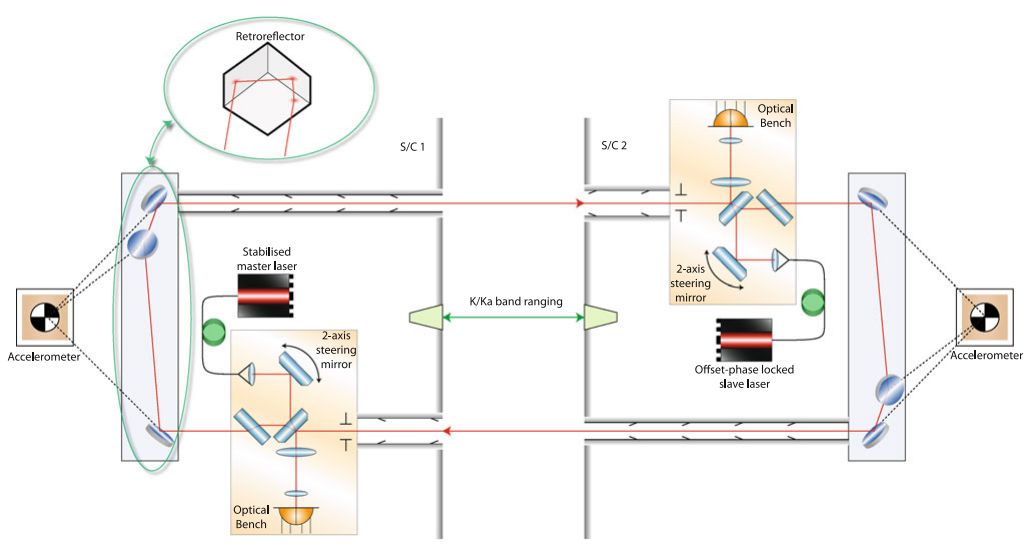
\includegraphics[height=0.7\textheight]{..//images//diagram_grace_fo.png}
    \end{figure}

\end{frame}

\begin{frame}{Key elements and TMA}
	\begin{block}{Key words}
		\textbf{off-axis, racetrack, three mirror assembly(TMA), Retro-reflector, vertex, transponder}
	\end{block}
	
	\begin{block}{TMA, retro-reflector}
		\begin{columns}
			\column{4cm}
			\begin{figure}
				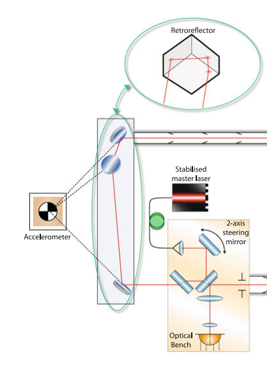
\includegraphics[height=0.5\textheight]{..//images//retroreflector.png}
			\end{figure}
			\column{8.5cm}
			$\Longrightarrow$ \textbf{Assumptions:}
			\begin{itemize}
				\item Three mirrors perpendicular to one another.
				\item Vertex of the retro-reflector is outside.
				\item Pathlength is twice than the distance $\dots$
				\item Two beams is \textbf{anti-parallel}.
				\item Lateral offsets are the same.
			\end{itemize}
		\end{columns}
	\end{block}
\end{frame}

\begin{frame}{Transponder}
	\begin{block}{Why the transponder exists???}
		Since the core of the two-ranging system is the transmitting satellite is the one to receive, why bother to arrange a slave transponder in the tracking satellite???
	\end{block}

	\begin{block}{Concerns}
		According to the fourth assumption of the last slide, the transmitting beam is anti-parallel to the receiving one. But the separation of the two GRACE FO satellites is so large so that this assumption cannot be taken unless the attitude of the two satellites can be sufficiently controlled. Unfortunately, the test illustrates it is not gonna happen.
	\end{block}
\end{frame}

\begin{frame}{Two-way ranging for GRACE-FO: Off-axis and racetrack}
	\begin{block}{Alas! The laser axis has been \textbf{BLOCKED}!}
		\begin{itemize}
			\item Continuing the design style of the GRACE, the KBR phase centre and cold gas tank are placed right in the centre of the front of the satellite.
			\item The shift offset cannot be too large in case that the error of attitude noise aligned into the range.
		\end{itemize}
		\begin{columns}
			\column{6cm}
			\begin{figure}
				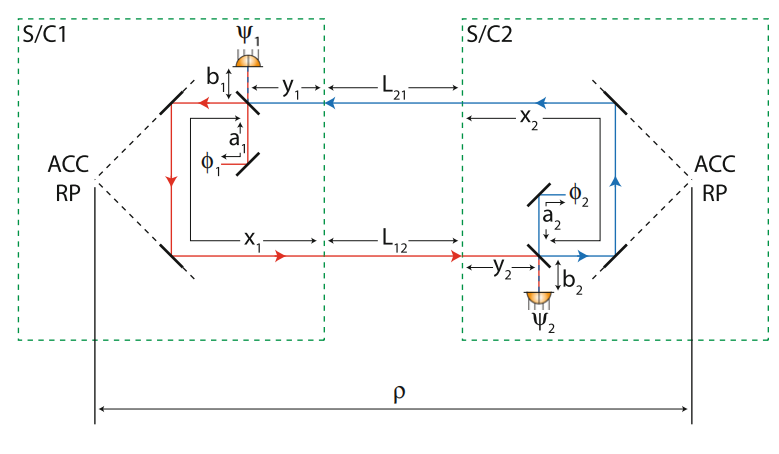
\includegraphics[height=3.3cm]{..//images//two_way_range_gracefo.png}
			\end{figure}
			\column{5cm}
			\begin{scriptsize}
				\begin{equation}
				\begin{split}
				\rho \left( t \right) \approx \frac{1}{2} [ x_1\left( t \right) +L_{12}\left( T \right) 
				 +y_2\left( t \right)\\
				  +L_{21}\left( t \right) 
				  +x_2\left( t \right) +y_1\left( t \right) ] 
				\end{split}
				\end{equation}
			\end{scriptsize}
		\end{columns}
		
	\end{block}
\end{frame}

\begin{frame}{Noise sources}
	\begin{block}{According to Sheard}
		\begin{itemize}
			\item \textbf{Two dominant sources:} pointing-induced noise, laser frequency noise
			\item \textbf{Other sources:} USO, shot, laser power, photodetector noise $\dots$
		\end{itemize}
	\end{block}

	\begin{block}{According to Vitali}
		\begin{itemize}
			\item laser frequency noise
			\item triple mirror assembly pointing jitter coupling
			\item additional linear and quadratic pointing jitter coupling
		\end{itemize}
	\end{block}
\end{frame}

\subsection{\hfill{}1.2. Organise GRACE-FO 1B data \hfill{}}

\begin{frame}{"Technical job" $\dots$}
	\begin{block}{Tools used}
		Python package: dask, one parallel and efficient package to handle large dataframes.
		
		Python library, documents at
		\href{https://SMPyBandits.GitHub.io}{\texttt{https://docs.dask.org/en/latest/}}
	\end{block}

	\begin{block}{Results}
		\textbf{Input} $\Longrightarrow$ the raw data of GRACE-FO 1B for Arbitrary days
		
		\textbf{Output} $\Longrightarrow$ the united dataframe for those days
		
		The same procedure as pre-processing Taiji-01
	\end{block}
\end{frame}

\subsection{\hfill{}1.3. KBR error propagation \hfill{}}

\begin{frame}{KBR error propagation}
	Good lord! Brought it off at last!!!
	\begin{block}{The error propagation formula}
		\begin{equation}
			\sigma _{n}^{2}\left( \delta T \right) =\frac{1}{1-P_n\left( cos\theta \right)}\frac{R_e}{GM}\left( \frac{r}{R_e} \right) ^{2n+1}\sigma _{n}^{2}\left( \delta \dot{\rho} \right) 
		\end{equation}
	\end{block}
	
	\begin{block}{The noise sources of KBR ranging}
		\begin{itemize}
			\item USO frequency shift
			\item System noise
			\item Take the above two as a whole
			\item Mutipath noise
		\end{itemize}
	\end{block}
\end{frame}

\begin{frame}{Degree error}
	Range-rate noise caused by USO frequency shift and system noise
	
	\begin{figure}
		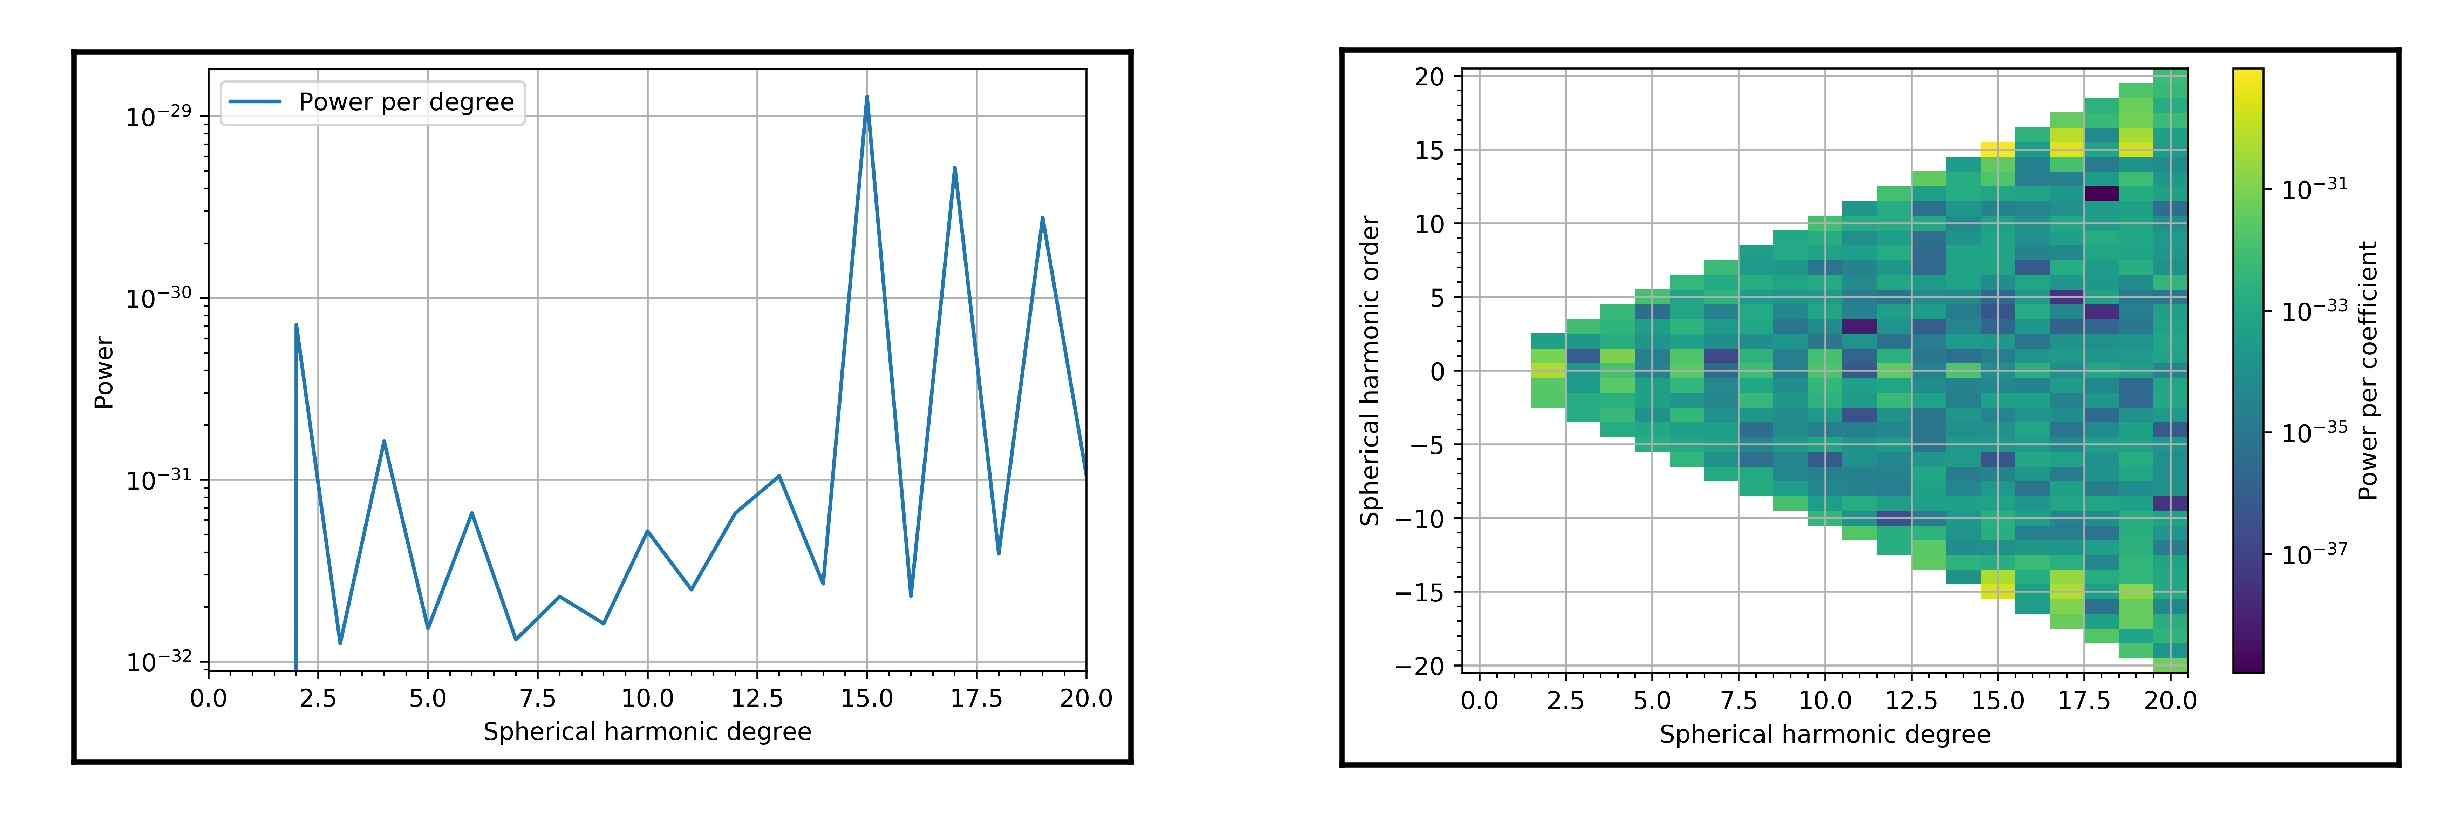
\includegraphics{..//images//kbr_os_sy.jpg}
	\end{figure}
\end{frame}

\begin{frame}{A small episode: Range}
	Since the arbitrary-days-long data is available,  the multipath noise went into a different situation.
	
	\begin{figure}
		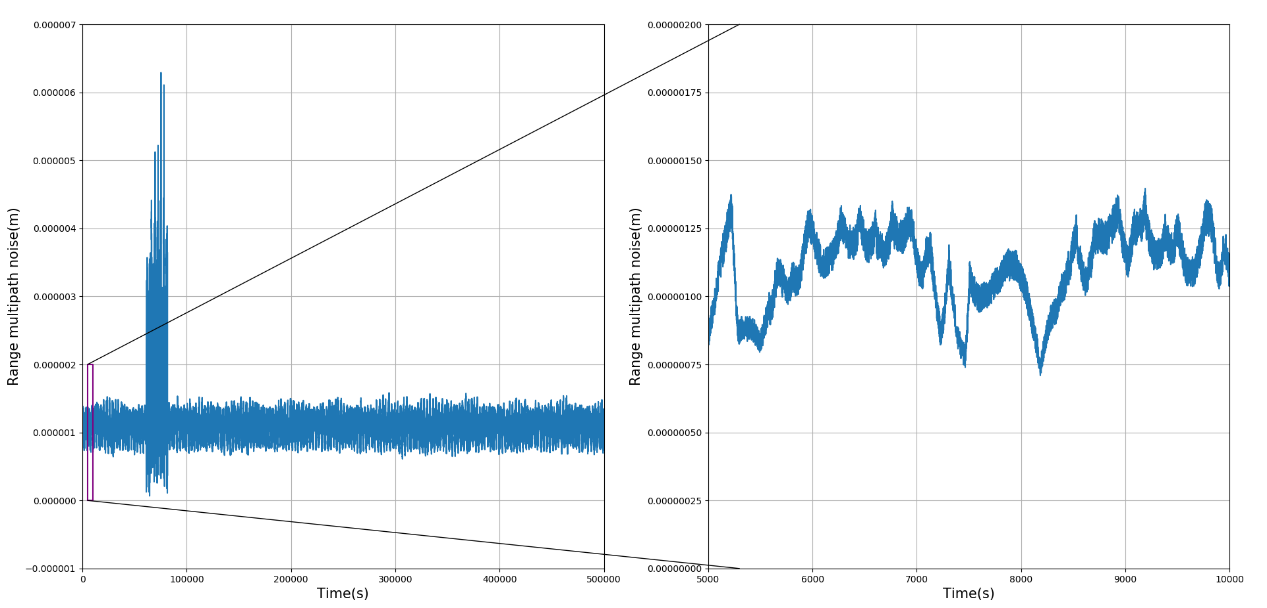
\includegraphics[height=0.5\textheight]{..//images//multipath_range_time.png}
		\caption{Range noise because of multipath noise (20190101-20190131)}
	\end{figure}
\end{frame}

\begin{frame}{A small episode: Range-rate}
	\begin{figure}
		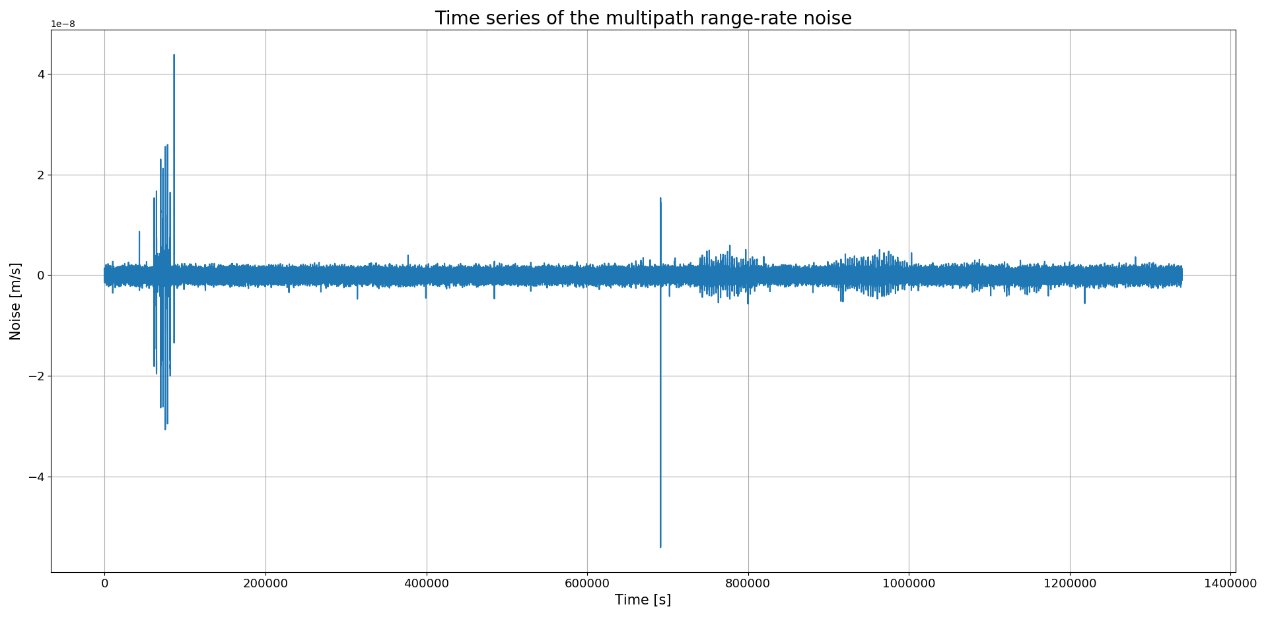
\includegraphics{..//images//multipath_range_rate_time.png}
		\caption{Range-rate noise because of multipath noise (20190101-20190131)}
	\end{figure}
\end{frame}

\begin{frame}{A small episode: PSD}
	\begin{figure}
		\subfigure{
		\begin{minipage}[t]{0.5\linewidth}
			\centering
			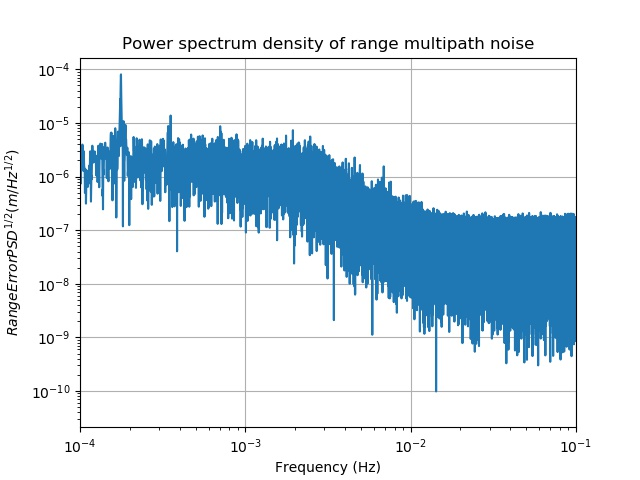
\includegraphics{..//images//psd_range_multipath_noise.jpg}
		\end{minipage}%
		}%
		\subfigure{
		\begin{minipage}[t]{0.5\linewidth}
			\centering
			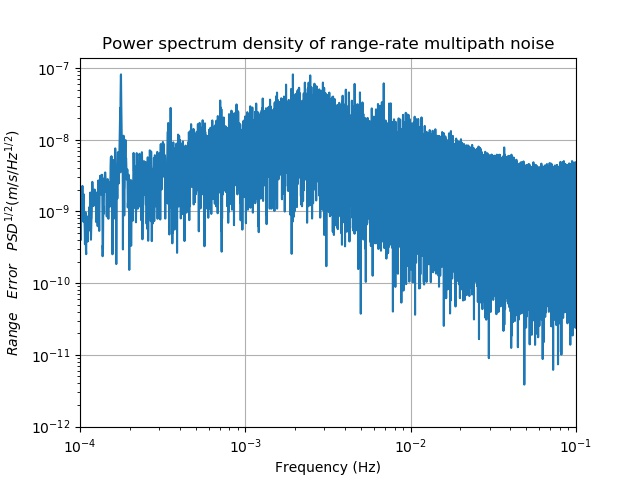
\includegraphics{..//images//psd_range_rate_multipath_noise.jpg}
		\end{minipage}%
		}
		\caption{PSD of multipath range and range-rate noise}
	\end{figure}
\end{frame}

\begin{frame}{Degree error}
	Degree error because of multipath noise.
	\begin{figure}
		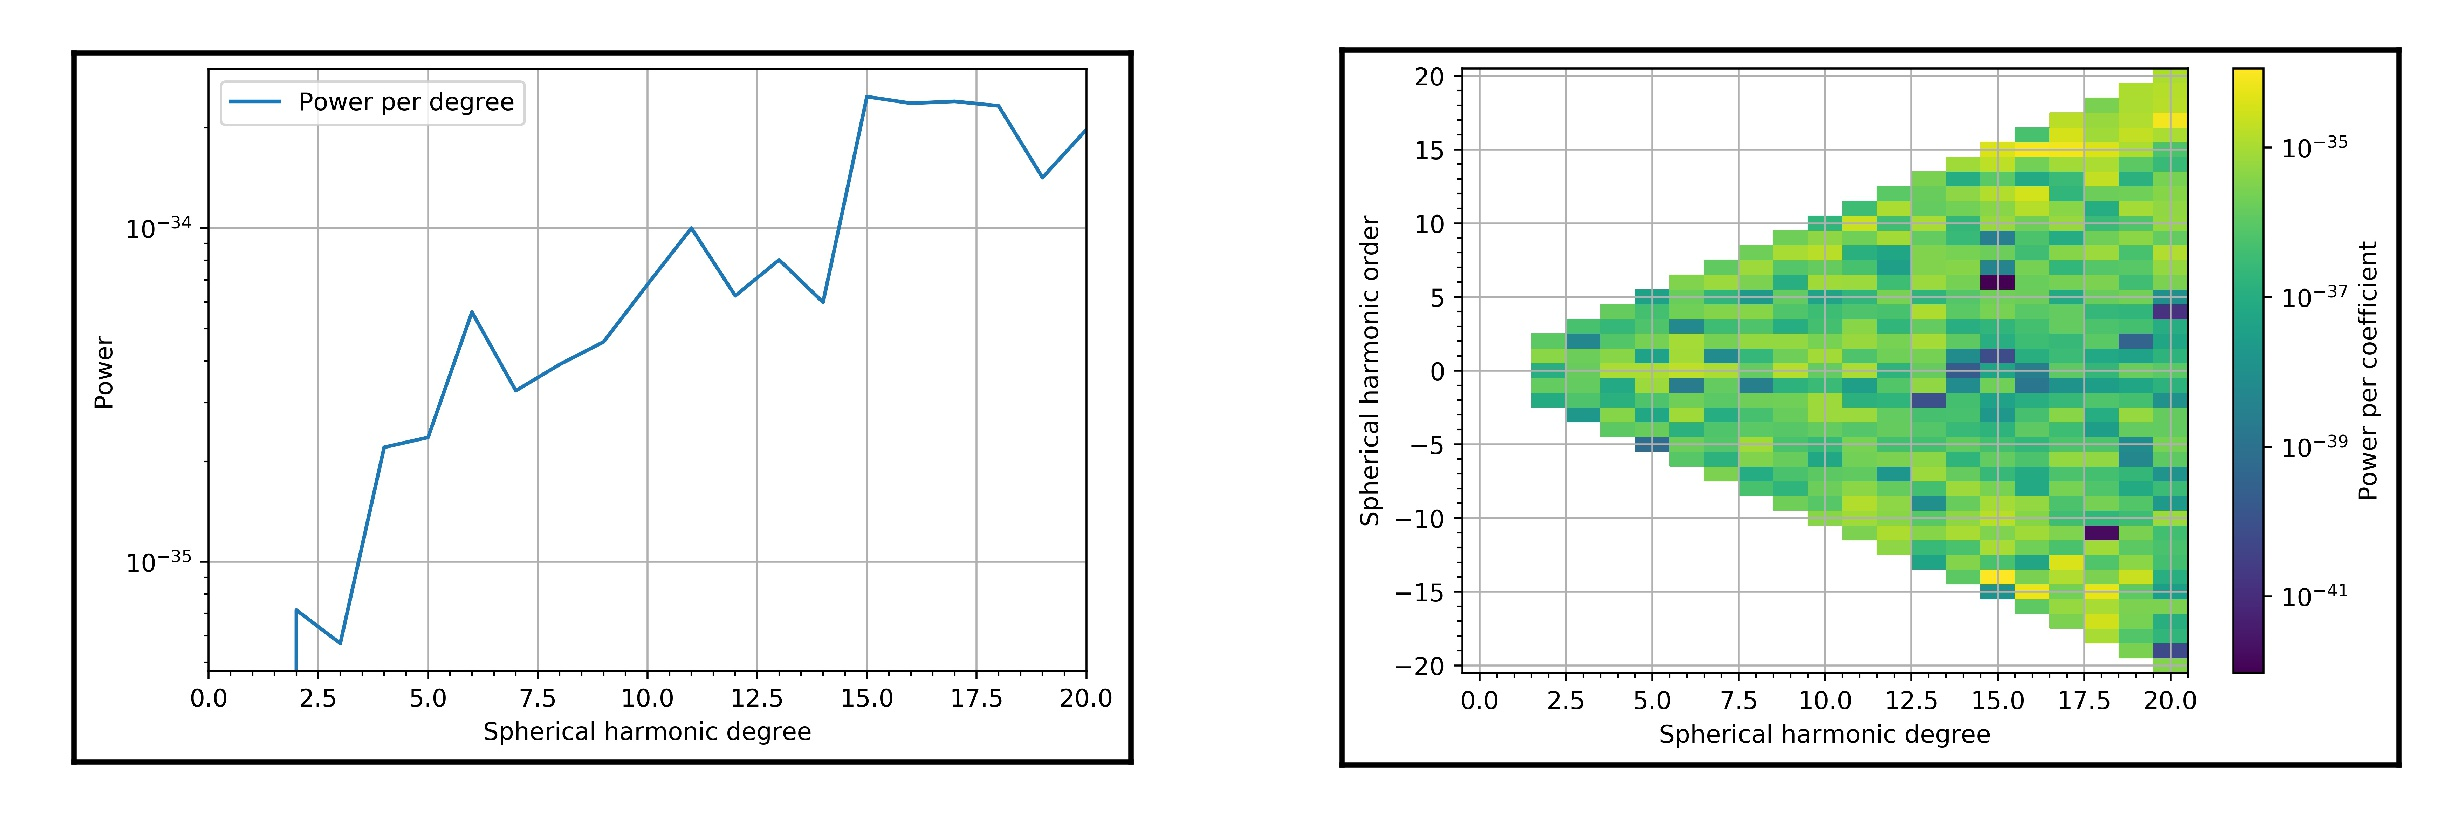
\includegraphics{..//images//kbr_multipath.jpg}
	\end{figure}
\end{frame}

\begin{frame}{Degree error}
	Total degree error of KBR ranging
	
	\begin{figure}
		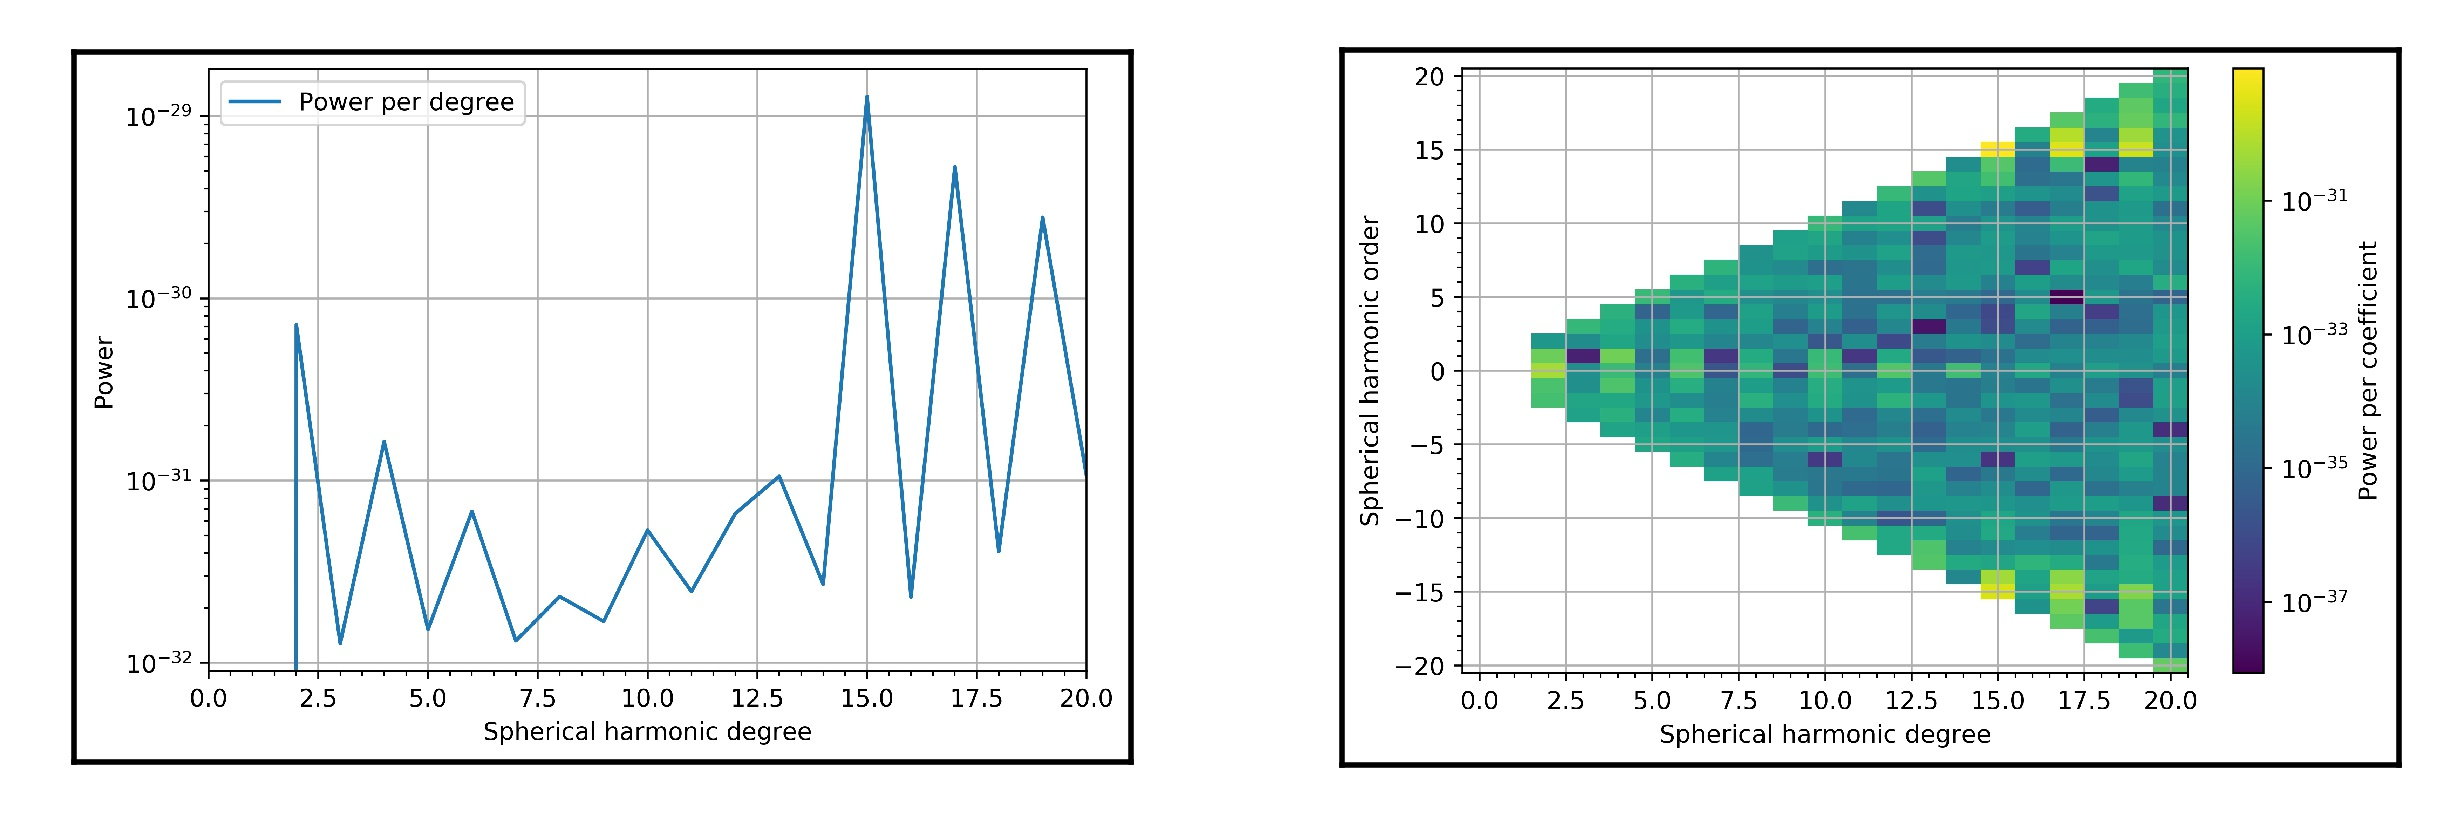
\includegraphics{..//images//kbr.jpg}
	\end{figure}

	The magnitude of the range-rate noise by USO frequency shift and system noise is much larger than the one caused by multipath noise.
\end{frame}

\subsection{\hfill{}1.4. Laser frequency noise model \hfill{}}

\begin{frame}{Filter to generate noise}
	\begin{block}{Formula $\Longrightarrow$ ASD}
		According to the cavity test of JPL, the ASD of the range noise because of laser frequency noise is as follows:
		
		\begin{equation}
			\bar{\delta}_{\rho LF}( f ) =5\times 10^{-9}\sqrt{1+\left( \frac{0.0182Hz}{f} \right) ^2}\frac{m}{\sqrt{Hz}}
		\end{equation}
	\end{block}
	\begin{block}{Formula $\Longrightarrow$ Time series}
		According to Sheard, the coupling of laser frequency noise into the range measurement is proportional to the satellite separation.
		
		\begin{equation}
			\delta _{\rho LF}( t ) =\frac{\rho}{238}\times \mathcal{F}^{-1}( 5\times 10^{-9}\sqrt{1+( \frac{0.0182Hz}{f} ) ^2}\frac{m}{\sqrt{Hz}}) 
		\end{equation}
	\end{block}
\end{frame}

\begin{frame}{PSD of range and range-rate noise}
	\begin{equation}
		\bar{\delta}_{\dot{\rho}LF}=2\pi f\bar{\delta}_{\rho LF}
	\end{equation}
	\begin{figure}
		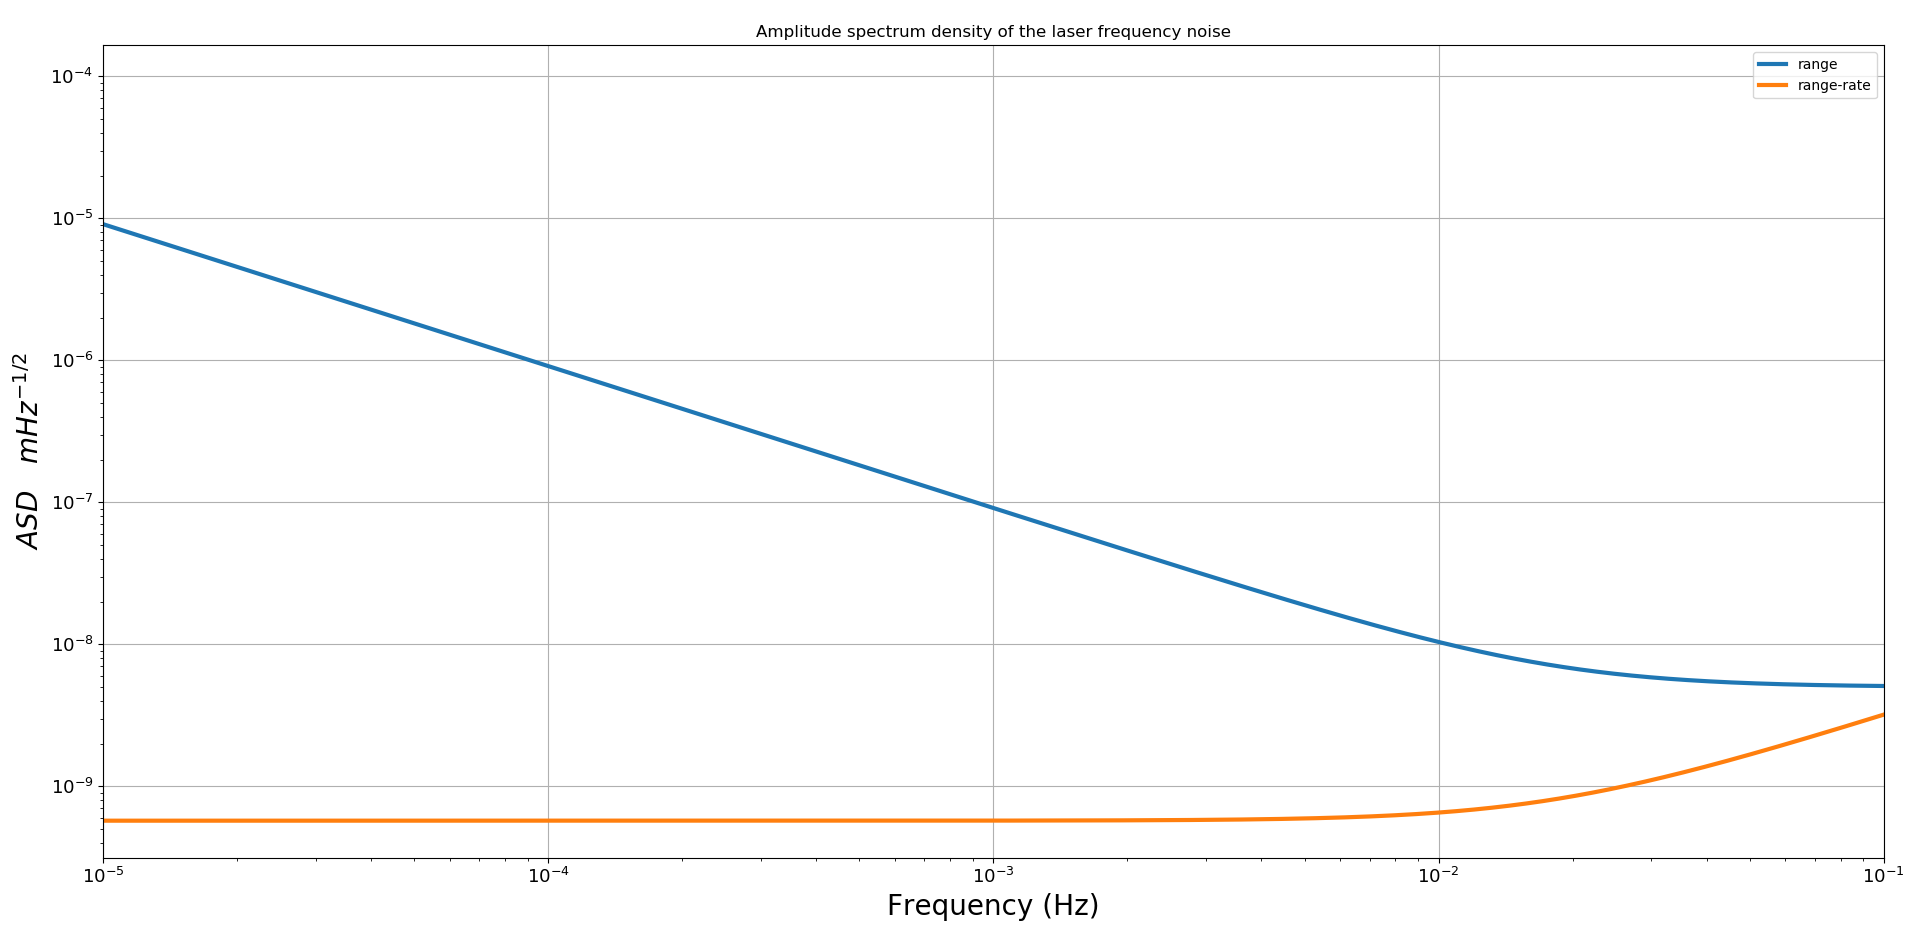
\includegraphics{..//images//laser_frequency_spectrum.png}
	\end{figure}
\end{frame}

\begin{frame}{Time series of range rate}
	Filtering approach as always $\dots$
	\begin{figure}
		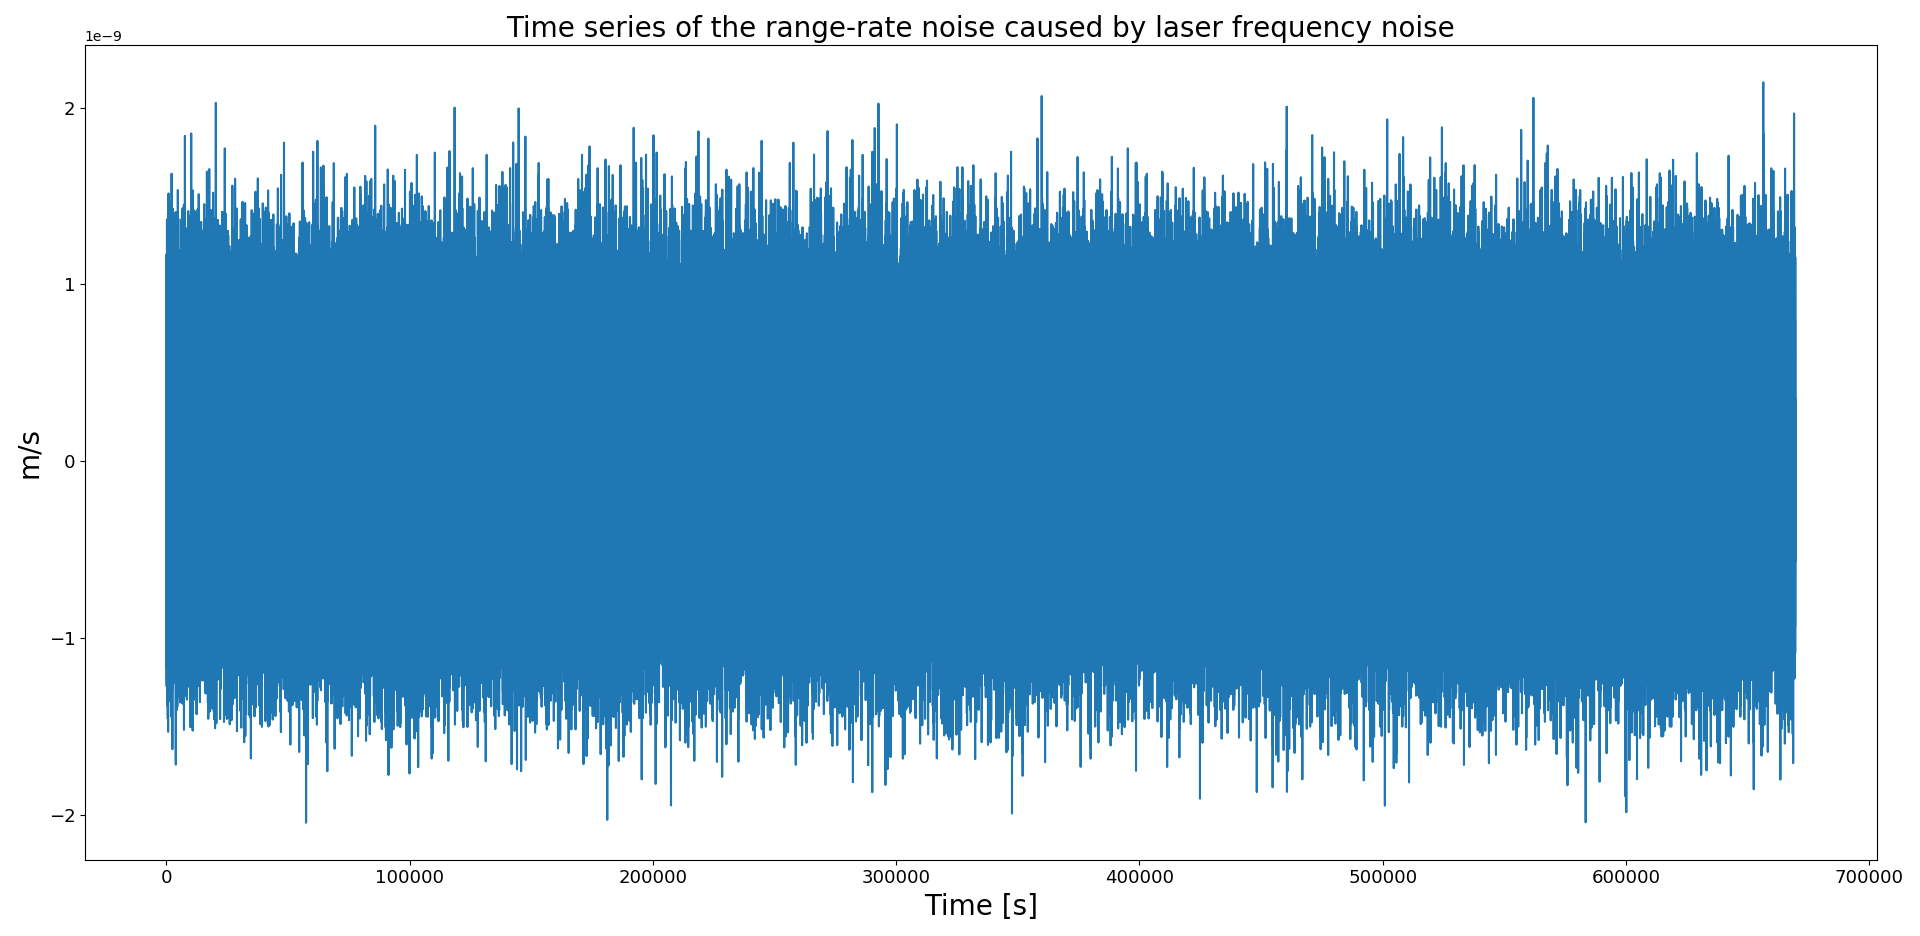
\includegraphics{..//images//filtered_range_rate.png}
	\end{figure}
\end{frame}

\subsection{\hfill{}1.5. Satellite's attitude in SRF \hfill{}}
\begin{frame}{Another two noise for LRI}
	\begin{block}{Triple mirror assembly poiting jitter coupling}
		\begin{equation}
			\delta \rho_{T M A_{A}}=-\left(e_{A B}^{I C R F}\right)^{T} \cdot \mathbf{R}_{S F}^{I C R F} \cdot \boldsymbol{v}_{A}^{S F}
		\end{equation}
	\end{block}
	\begin{block}{Additional linear and quadratic pointing jitter coupling}
		\begin{tiny}
		\begin{equation}
		 \delta \rho _{ALQ_A}=\left[ \begin{matrix}
		 c_{x_A}&		c_{y_A}&		c_{z_A}\\
		 \end{matrix} \right] \cdot \left[ \begin{array}{c}
		 \theta _{x_A}\\
		 \theta _{y_A}\\
		 \theta _{z_A}\\
		 \end{array} \right] +\left[ \begin{matrix}
		 \theta _{x_A}&		\theta _{y_A}&		\theta _{z_A}\\
		 \end{matrix} \right] \cdot \left[ \begin{matrix}
		 c_{xx_A}&		c_{xy_A}&		c_{xz_A}\\
		 0&		c_{yy_A}&		c_{yz_A}\\
		 0&		0&		c_{zz_A}\\
		 \end{matrix} \right] \cdot \left[ \begin{array}{c}
		 \theta _{x_A}\\
		 \theta _{y_A}\\
		 \theta _{z_A}\\
		 \end{array} \right] 
		\end{equation}
		\end{tiny}
	\end{block}

	\begin{block}{Interpretation}
		$\mathbf{R}_{S F}^{I C R F}$  is the transformation matrix from SF into ICRF; $\theta _{x_A}$ is the roll angle for GRACE-FO C.
	\end{block}
\end{frame}

\begin{frame}{Transformation matrix}
	According to Vilali and spiceypy, 
	\begin{block}{The matrix rotating from SF into ICRF is related to the quaternions by:}
		\begin{tiny}
		\begin{equation}
			\mathbf{R}_{S F}^{I C R F}=\left[\begin{array}{ccc}
			q_{0}^{2}+q_{1}^{2}-q_{2}^{2}-q_{3}^{2} & 2\left(q_{1} q_{2}-q_{0} q_{3}\right) & 2\left(q_{1} q_{3}+q_{0} q_{2}\right) \\
			2\left(q_{1} q_{2}+q_{0} q_{3}\right) & q_{0}^{2}-q_{1}^{2}+q_{2}^{2}-q_{3}^{2} & 2\left(q_{2} q_{3}-q_{0} q_{1}\right) \\
			2\left(q_{1} q_{3}-q_{0} q_{2}\right) & 2\left(q_{2} q_{3}+q_{0} q_{1}\right) & q_{0}^{2}-q_{1}^{2}-q_{2}^{2}+q_{3}^{2}
			\end{array}\right]
		\end{equation}
		\end{tiny}
	\end{block}

	\begin{block}{The matrix rotating from ICRF into LOSF is derived from the orbital positions:}
		\begin{tiny}
			\begin{equation}
			\mathbf{R}_{I C R F}^{L O S F}=\left[\boldsymbol{x}_{L O S F}, \boldsymbol{y}_{L O S F} , \boldsymbol{z}_{L O S F}\right]
			\end{equation}
			\begin{equation}
				\theta_{x}=\arctan (\frac{R_{32}}{R_{33}});
				\theta_{y}=-\arcsin (R_{31});
				\theta_{z}=\arctan (\frac{R_{21}}{R_{11}})
			\end{equation}
			\begin{equation}
				\boldsymbol{x}_{L O S F_{A}}=\frac{\boldsymbol{r}_{B}-\boldsymbol{r}_{A}}{\left|\boldsymbol{r}_{B}-\boldsymbol{r}_{A}\right|};
				\boldsymbol{y}_{L O S F_{A}}=\frac{\boldsymbol{x}_{L O S F_{A}} \times \boldsymbol{r}_{A}}{\left|\boldsymbol{x}_{L O S F_{A}} \times \boldsymbol{r}_{A}\right|};
				z_{L O S F_{A}}=\boldsymbol{x}_{L O S F_{A}} \times \boldsymbol{y}_{L O S F_{A}}
			\end{equation}
		\end{tiny}
	\end{block}
\end{frame}


\begin{frame}{Bad news $\dots$}
	\begin{figure}
		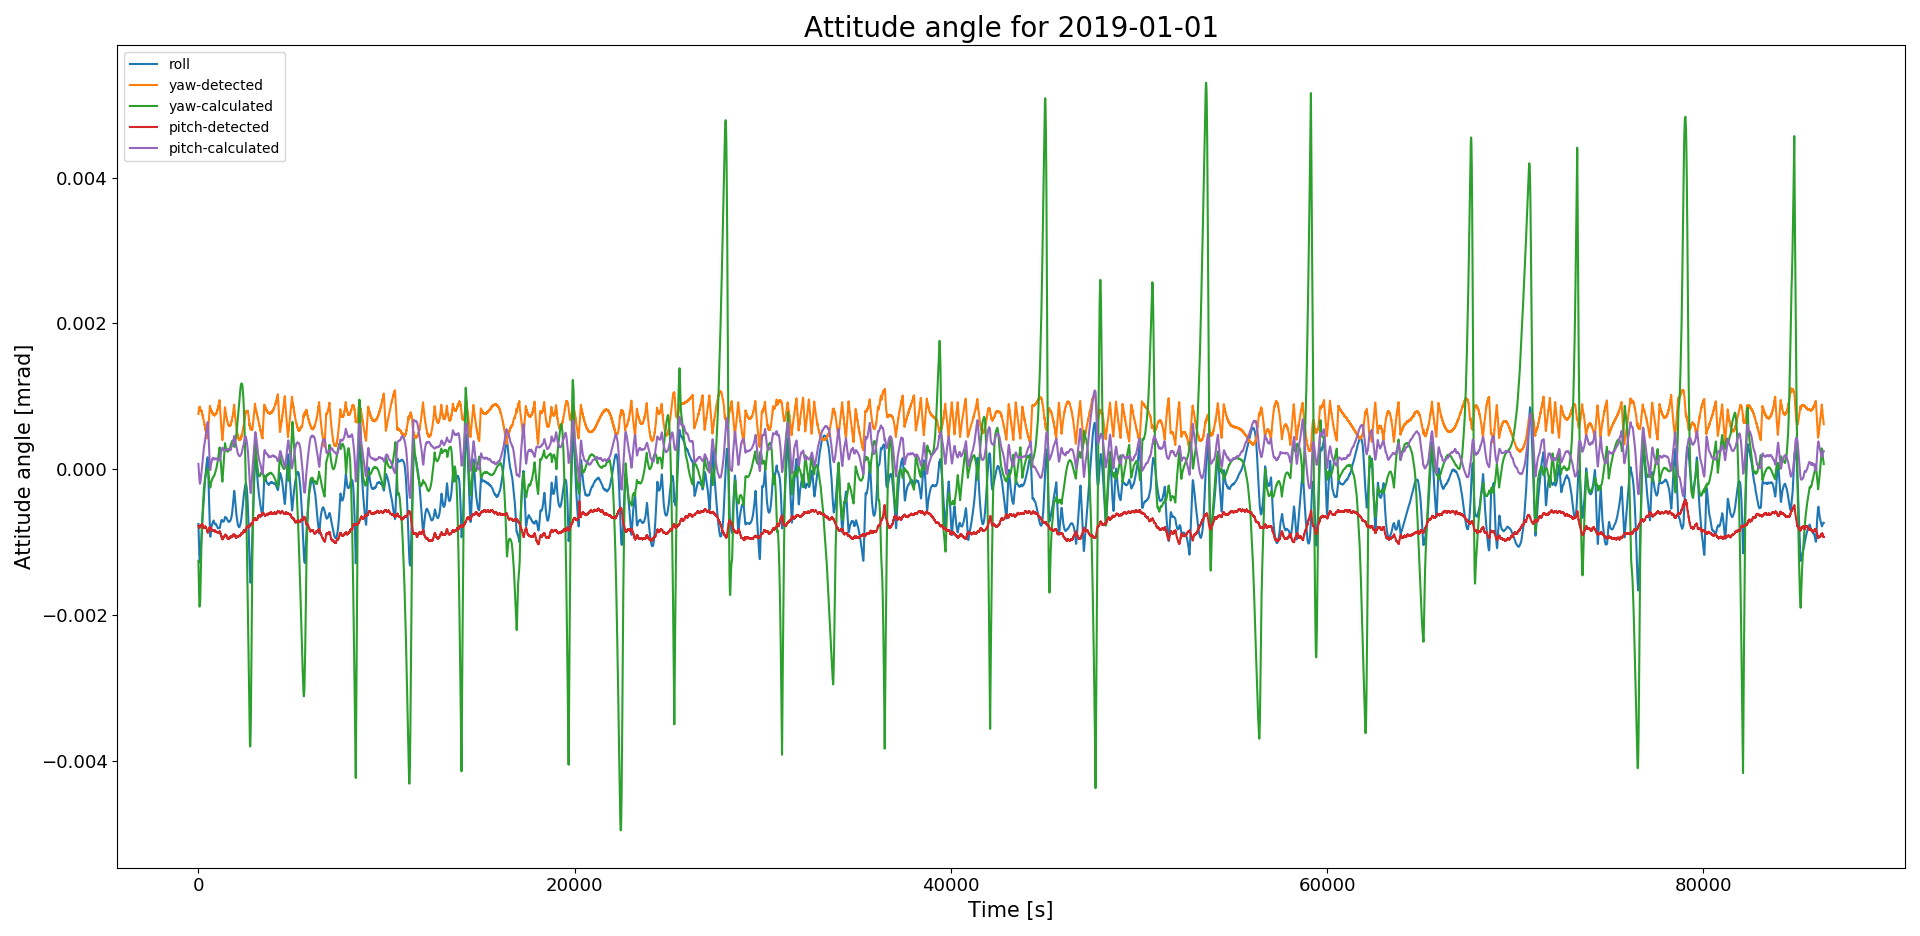
\includegraphics[height=0.5\textheight]{..//images//attitude_angle_2019_01_01.png}
	\end{figure}
	\begin{block}{Big difference}
		The yaw attitude angle is completely different.
		
		Tried several rotating method, it is the one that is most correct.
		
		Still don't know how to fix it.
	\end{block}
\end{frame}


\section{\hfill{}2. Arrangement for next week\hfill{}}
\subsection{\hfill{}2.1. Finish the laser ranging model and error propagation\hfill{}}
\begin{frame}{LRI noise model}
	\begin{block}{Obstacles}
		\begin{itemize}
			\item The attitude angle
		\end{itemize}
	\end{block}
	\begin{block}{Wish to accomplish}
		\begin{itemize}
			\item Model of LRI noise model
			\item Error propagation of LRI
			\item Plotting all diagrams
		\end{itemize}
	\end{block}
	\begin{block}{Tools}
		\begin{itemize}
			\item Astropy
			\item Spiceypy
		\end{itemize}
	\end{block}
\end{frame}

\subsection{\hfill{}2.2. Revise all the fortran program into module-style\hfill{}}
\begin{frame}{Module Style}
	\begin{block}{Problems met}
		Hard to manage hundreds even thousands of variables and dozens of subtoutines
		
		Printing report seems to be a problem
	\end{block}
	\begin{block}{Advantages}
		\begin{itemize}
			\item Better encapsulation
			\item Objective-oriented
			\item More easy to manage variables and subroutines
		\end{itemize}
	\end{block}
\end{frame}

\section{Thanks!}


\begin{frame}
	\centering
	
	\begin{spacing}{2}
	\begin{Huge}
		Thanks for listening!\\
	\end{Huge}
	\end{spacing}
	\begin{spacing}{3}
		
	\end{spacing}
	\textbf{Hao-si Li}\\
	Sichuan - 27th March 2020\\
		
	
\includegraphics[height=0.16\textheight]{../common/logo_chd.png}
	
\includegraphics[height=0.16\textheight, width=0.6\linewidth]{../common/log_tiji.jpg}
		
\end{frame}

\end{document}
